\documentclass{article}
\usepackage{graphicx}
\usepackage{listings}
\usepackage{xcolor}
\usepackage{amsmath}
\usepackage[a4paper, margin=1in]{geometry}
\setlength{\parindent}{0pt}

\title{Week8 Lab1 Report}
\author{111062117, Hsiang-Sheng Huang}

\begin{document}

\maketitle

\section*{1. Identify Top MPI Functions}

List the top three MPI functions that consume the most time in the application. Provide a brief explanation for why you think these functions are the most time-consuming.

\begin{enumerate}
    \item \texttt{MPI\_File\_open}: Time-consuming due to coordination overhead between processes accessing the file system in parallel.
    \item \texttt{MPI\_Allreduce}: Requires synchronization and data exchange among all processes, creating communication bottlenecks, especially with large data.
    \item \texttt{MPI\_File\_close}: Involves synchronization to ensure all processes have completed their I/O operations before closing the file.
\end{enumerate}

\begin{figure}[h]
    \centering
    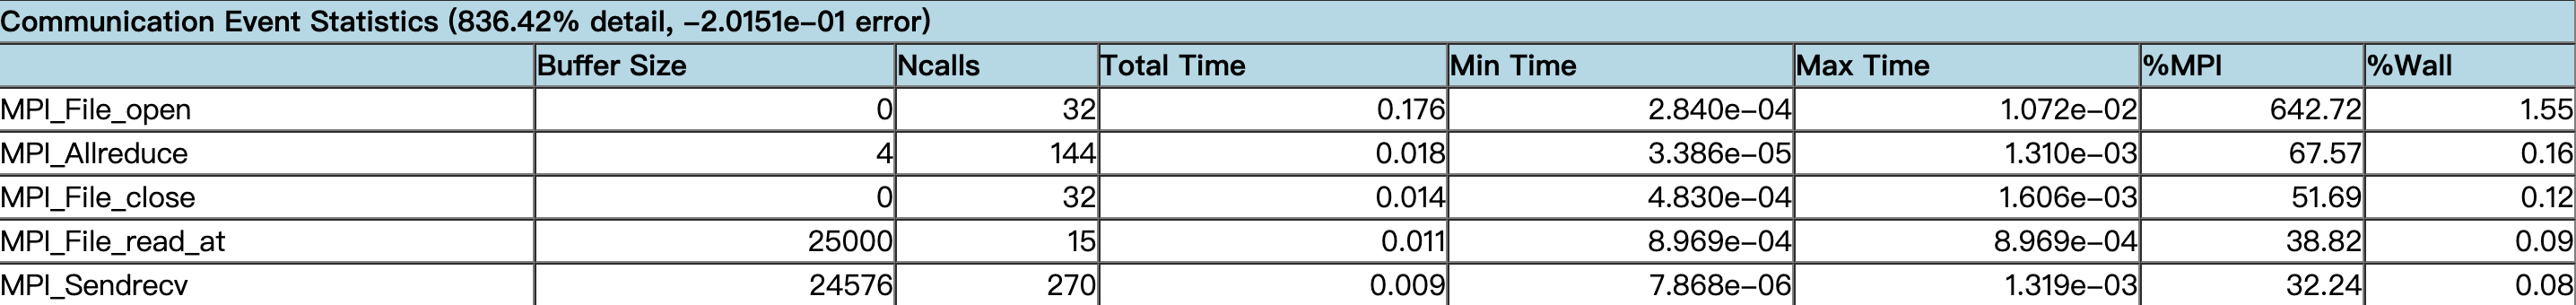
\includegraphics[width=1\textwidth]{./img/q1.png}
    \caption{Top MPI Functions}
\end{figure}

\section*{2. Visualization}

Paste the pie chart generated by the IPM profiler that illustrates the time distribution across different MPI functions in your application.

\begin{figure}[h]
    \centering
    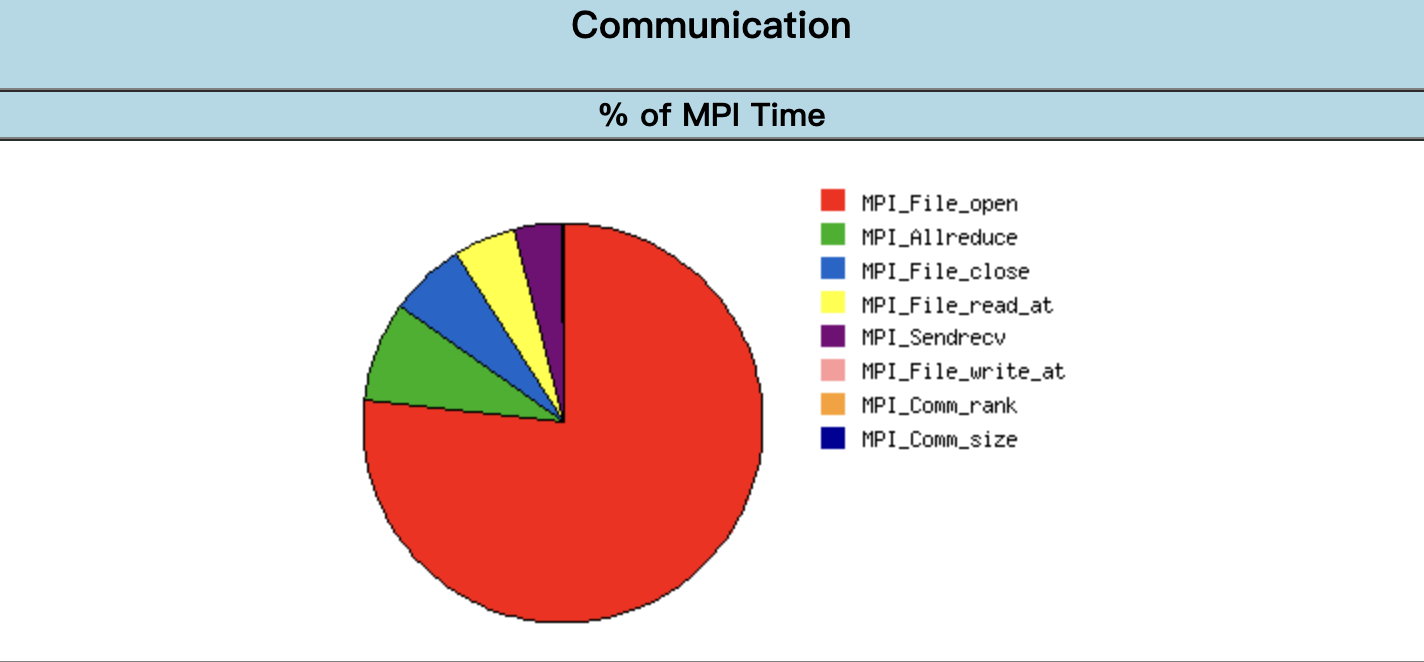
\includegraphics[width=0.8\textwidth]{./img/q2.png}
    \caption{MPI Function Time Distribution}
\end{figure}

\end{document}
